%\section{Results}

%In this section, we analyze the quality of results considering the $C_{max}$ values obtained for each DE algorithm described in Section~\ref{sec:HDE} to solve the FSSSP instances. 

\section{Experimental Results}% of DE and Different CR Values}
\vspace{-0.4cm}
The first analysis is focused on the effect of using different $Cr$ values in the DE performance, from low to high values (0.1, 0.5 and 0.9). %For that purposes, we analyze the quality of results considering the $C_{max}$ values obtained for the basic DE algorithm to solve the FSSSP instances. 
Table \ref{tab:resultsDE} shows the best $C_{max}$ values obtained for the DE algorithm using the different $Cr$ values for each instance (columns 3 to 5). Also, the mean $C_{max}$ values together with the mean standard deviation (sd) are presented (columns 6 to 8). Column 2 displays the best known $C_{max}$ value for each instance. Last column shows the results of the KW test, where
the symbol ``+'' indicates significant differences between the algorithms ( $p$-value is inferior to the significance  level$\alpha$ = 0.01). %Lowest values of $gap_{meanBest}$ indicates that the algorithm is able to find the best $C_{max}$ values for the majority of the runs. 

The DE algorithm with $Cr$=0.9 finds lowest $C_{max}$ values than the rest. Moreover, this configuration reaches the best known $C_{max}$ values in 5 of the 10 instances. Now, analyzing what is happening with the mean $C_{max}$ values, the DE using $Cr$=0.1 presents the lowest values for the four first instances (MK01-04). Furthermore, sd values are equal to zero for these instances, indicating that the algorithm is able to find the optimum value for all the runs. In the remaining instances (MK05-10), the DE with $Cr$=0.9 presents the lowest $C_{max}$ values. Finally, the DE using $Cr$=0.5 shows the worst performance. Given that the $p$-values of KW test is lower than the level of significance considered, we can state that there are significant differences among the DE with $Cr$ values (except for instances MK01, MK03, and MK08).  %A complementary information to the previous analysis is shown in Figure~\ref{fig:DEhitRate}, which presents the hit rate obtained for the DE and each Cr value. This metric measures the number of times the algorithm finds the optimal value in the 30 executions performed by the DE for each Cr value. These results support the previous analysis. 

From previous analysis, we can conclude that for instances with relatively few operations, the fraction of parameter values that are copied from the target vector in the recombination operation should be small to allow the algorithm to find the best solutions to the problem. On the other hand, when the complexity of the instances grows up, it is necessary to increase the amount of disturbances in the solutions, and in this way the algorithm could converge to near-optimal solutions. Consequently, we will adopt two different values of $Cr$ for the remaining experimentation: $Cr$ = 0.1 for MK01-04 instances and $Cr$ = 0.9 for the remaining ones. 

%Finally, we proceed to study the distribution of the number of evaluations to find the best $C_{max}$ value performed by DE with different Cr values. For that purpose, Figure~\ref{fig:DEevaluations}  illustrates these results by means of two box-plot graph. The one on the left are devoted to the less complex instances MK01-04, whereas the other one presents the distribution for the remaining instances. We observe that the DE algorithm with more evaluations is the one with Cr=0.1, although this approach outperforms the other ones from the result quality point of view (see Table~\ref{tab:DE} for the MK01-04 instances. In the rest of the instances, DE with Cr = 0.9 is faster the rest, regarding the number of evaluations to find the best $C_{max}$.

\begin{table}[!tb]
    \scriptsize
    \centering

    \caption{$C_{max}$ values found by the DE algorithm with different $Cr$ values% for all FJSSP instances
    .}
\begin{tabular}{|l|l|rrr|rrr|c|}
\hline
\multicolumn{1}{|c|}{\multirow{2}{*}{Instance}} & \multicolumn{1}{c}{\multirow{2}{*}{Opt.}} & \multicolumn{3}{|c|}{Best $C_{max}$ Values} & \multicolumn{3}{c|}{Mean $C_{max}$ Values  $_{\pm}$ sd} & \multicolumn{1}{c|}{\multirow{2}{*}{KW}}\\
\cline{3-8}
\multicolumn{1}{|c|}{} & \multicolumn{1}{c|}{} & \multicolumn{1}{|c}{$Cr$=0.1} & \multicolumn{1}{c}{$Cr$=0.5} & \multicolumn{1}{c|}{$Cr$=0.9} & \multicolumn{1}{c}{$Cr$=0.1} & \multicolumn{1}{c}{$Cr$=0.5} & \multicolumn{1}{c|}{$Cr$=0.91} &\\
\hline
    Mk01  & \textbf{40} & \textbf{40} & \textbf{40} & \textbf{40} & 40.00  $_{\pm 0.00   }$    & 40.00  $_{\pm 0.00   }$    & 40.73  $_{\pm 0.78   }$    & - \\
    Mk02  & 26    & 27    & 27    & 27    & 27.00  $_{\pm 0.00   }$    & 27.20  $_{\pm 0.42   }$    & 27.33  $_{\pm 0.47   }$    & + \\
    Mk03  & 204   & \textbf{204} & \textbf{204} & \textbf{204} & 204.00  $_{\pm 0.00   }$    & 204.00  $_{\pm 0.00   }$    & 204.00  $_{\pm 0.00   }$    & - \\
    Mk04  & 60    & \textbf{60} & 61    & \textbf{60} & 61.70  $_{\pm 0.60   }$    & 65.20  $_{\pm 2.53   }$    & 64.80  $_{\pm 2.19   }$    & + \\
    Mk05  & 172   & 174   & 177   & 173   & 175.87  $_{\pm 0.73   }$    & 181.10  $_{\pm 1.79   }$    & 174.03  $_{\pm 1.82   }$    & + \\
    Mk06  & 58    & 66    & 70    & 60    & 67.17  $_{\pm 0.59   }$    & 71.10  $_{\pm 0.74   }$    & 63.15  $_{\pm 1.12   }$    & + \\
    Mk07  & 139   & 144   & 149   & 140   & 144.07  $_{\pm 0.25   }$    & 150.10  $_{\pm 0.99   }$    & 142.18  $_{\pm 1.30   }$    & + \\
    Mk08  & 523   & \textbf{523} & \textbf{523} & \textbf{523} & 523.00  $_{\pm 0.00   }$    & 523.30  $_{\pm 0.95   }$    & 523.00  $_{\pm 0.00   }$    & - \\
    Mk09  & 307   & 321   & 338   & \textbf{307} & 325.13  $_{\pm 1.48   }$    & 343.00  $_{\pm 2.40   }$    & 310.05  $_{\pm 2.48   }$    & + \\
    Mk10  & 197   & 237   & 249   & 213   & 241.03  $_{\pm 1.25   }$    & 252.00  $_{\pm 1.25   }$    & 218.00  $_{\pm 2.71   }$    & + \\
\hline 
\end{tabular}
    \label{tab:resultsDE}
\end{table}


%\begin{figure}[!htb]
%\scriptsize
%\centering
%\begin{minipage}[b]{0.5\linewidth}
%    \centering
%    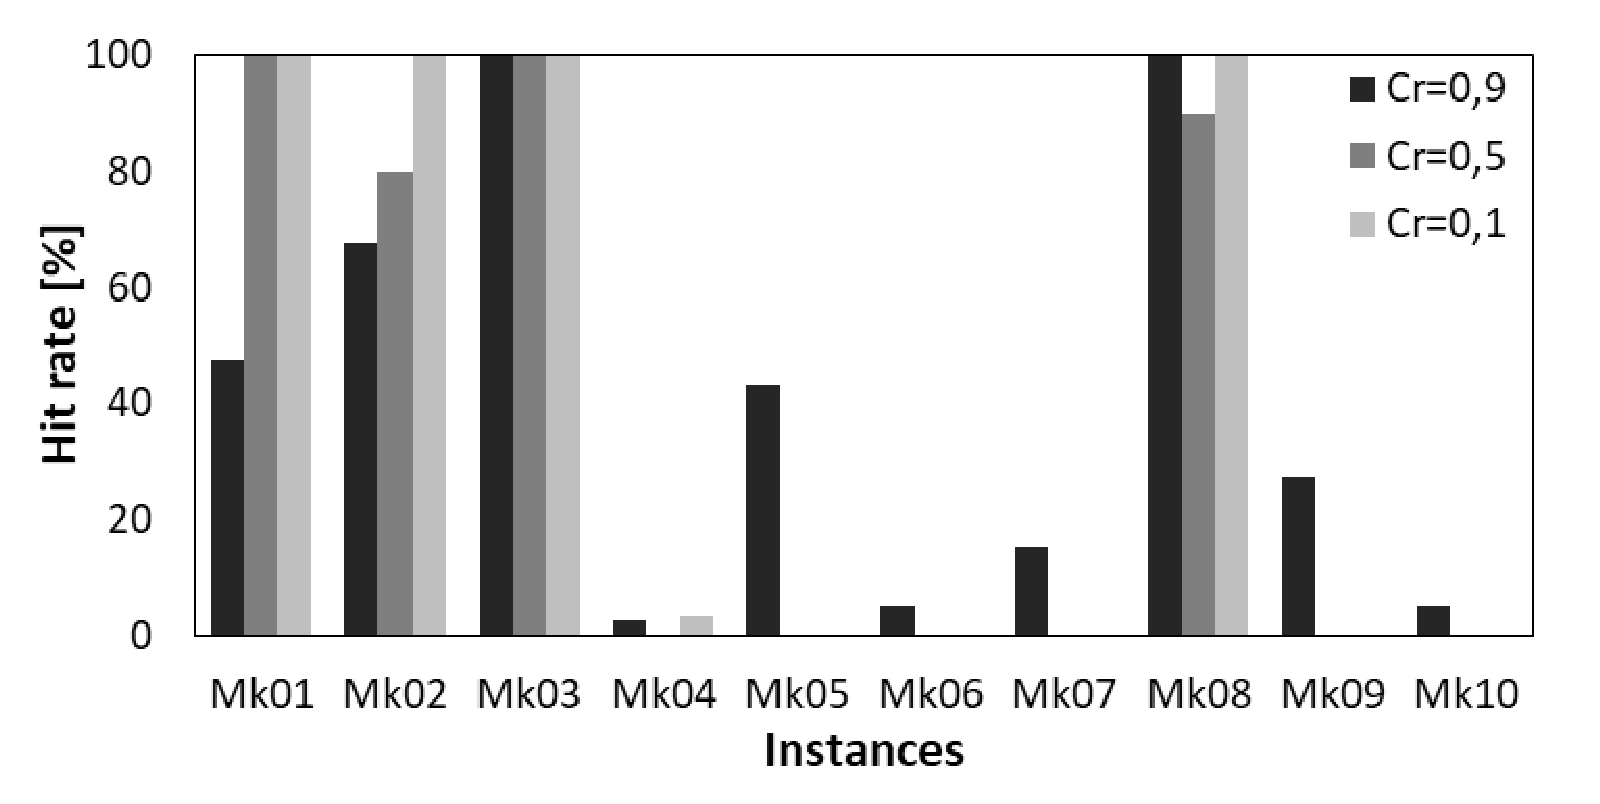
\includegraphics[width=0.75\textwidth]{figures/DE-hitRate.eps}
%    \caption{Hit Rate of the DE with different Cr values considering all FJSSP instances.}
%    \label{fig:DEhitRate}
%\end{minipage}  
%\hspace{0.5cm}
%\begin{minipage}[b]{0.5\linewidth}
%    \centering
%    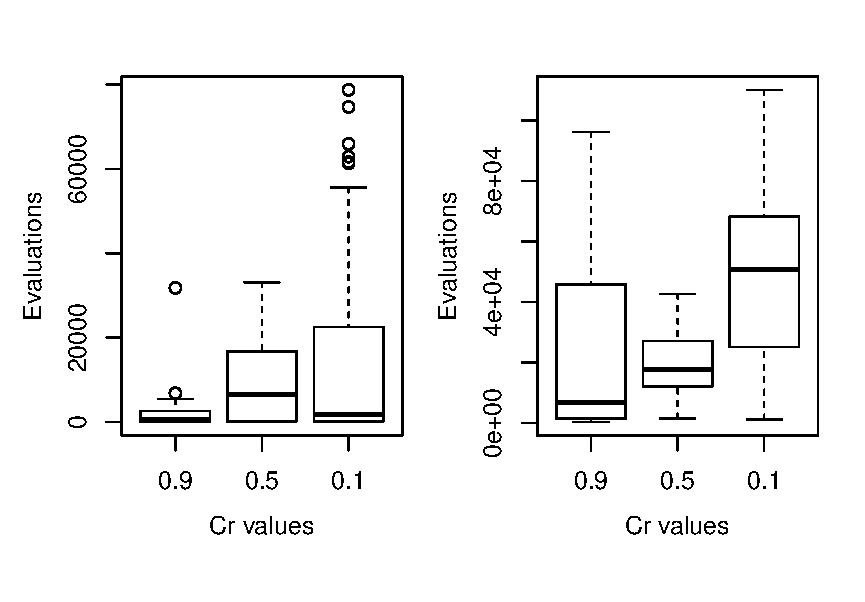
\includegraphics[width=0.75\textwidth]{figures/DE-Evaluations.eps}
%    \caption{Total number of evaluations done by running DE with different Cr values considering all FJSSP instances.}
%    \label{fig:DEevaluations}
%\end{minipage}
%\end{figure}


%\subsection{Results of the DE with Local Search}

Following analysis goes into detail of what happened with the introduction of a local search procedure to the DE algorithm (HDE) to solve the FJSSP. For that purpose, we considered three different $p_{LS}$ values: 0.1, 0.5 and 0.7 (low, medium, and high probability values), i.e. we study how the frequency of the LS application impacts on the DE performance.

Table~\ref{tab:HDE} shows the best and mean $C_{max}$ values obtained for the HDE with the different $p_{LS}$ values. The HDE algorithm applying the local search procedure with high frequency ($p_{LS}$=0.7) obtains low best $C_{max}$ values for the majority of the FJSSP instances. Moreover, this algorithm exhibits the lowest mean $C_{max}$ values for all instances. These indicate that the algorithm is able to find the optimum or the near-optimum values in the majority of the runs.  Moreover, the KW test indicates that there are statistical significant differences among the algorithms ($p$-values are lower than the level of significance). Comparing  $C_{max}$ values from Table~\ref{tab:resultsDE} and the ones from Table~\ref{tab:HDE}, we can observe that the HDE algorithms obtain best 

\begin{table}[!tb]
\scriptsize
\centering

\caption{$C_{max}$ values found by the HDE algorithm with different $p_{LS}$ values% for all FJSSP instances
.}
\begin{tabular}{|c|c|rrr|rrr|c|}
\hline
\multicolumn{1}{|c}{\multirow{2}{*}{Inst}} & \multicolumn{1}{|c}{\multirow{2}{*}{Opt.}} & \multicolumn{3}{|c}{Best $C_{max}$} & \multicolumn{3}{|c|}{Mean $C_{max}$ values $_{\pm}$ sd} &\multicolumn{1}{c|}{\multirow{2}{*}{KW}} \\
\cline{3-8}
\multicolumn{1}{|c}{} & \multicolumn{1}{|c|}{} &$p_{LS}$=0.1 & $p_{LS}$=0.5 & $p_{LS}$=0.7 & $p_{LS}$=0.1 & $p_{LS}$=0.5 & $p_{LS}$=0.7 & \multicolumn{1}{c|}{}\\
\hline
MK01 & 40 & \textbf{40} & \textbf{40} & \textbf{40} & 40.00  $_{\pm  0.00  }$ & 40.00  $_{\pm  0.00  }$ & 40.00  $_{\pm  0.00  }$ & -\\
MK02 & 26 & 27 & \textbf{26} & \textbf{26} & 27.00  $_{\pm  0.00  }$ & 26.80  $_{\pm  0.41  }$ & 26.77  $_{\pm  0.43  }$ & + \\
MK03 & 204 & \textbf{204} & \textbf{204} & \textbf{204} & 204.00  $_{\pm  0.00  }$ & 204.00  $_{\pm  0.00  }$ & 204.00  $_{\pm  0.00  }$ & - \\
MK04 & 60 & \textbf{60} & \textbf{60} & \textbf{60} & 61.20  $_{\pm  0.66  }$ & 60.33  $_{\pm  0.48  }$ & 60.17  $_{\pm  0.38  }$ & +\\
MK05 & 172 & 173 & 173 & 173 & 1.73  $_{\pm  0.18  }$ & 173.00  $_{\pm  0.00  }$ & 173.00  $_{\pm  0.00  }$ & +\\
MK06 & 58 & 62 & 61 & 60 & 63.27  $_{\pm  0.69  }$ & 62.13  $_{\pm  0.73  }$ & 61.90  $_{\pm  0.48  }$ & +\\
MK07 & 139 & 140 & \textbf{139} & 140 & 142.37  $_{\pm  0.96  }$ & 140.83  $_{\pm 0.79  }$ & 140.63  $_{\pm  0.61  }$ &+\\
MK08 & 523 & \textbf{523} & \textbf{523} & \textbf{523} & 523.00  $_{\pm 0.00  }$ & 523.00  $_{\pm  0.00  }$ & 523.00  $_{\pm  0.00  }$ &-\\
MK09 & 307 & \textbf{307} & \textbf{307} & \textbf{307} & 309.93  $_{\pm  1.53  }$ & 307.67  $_{\pm  1.06  }$ & 307.37  $_{\pm  0.89  }$ &+\\
MK10 & 197 & 225 & 223 & 219 & 228.20  $_{\pm  1.97  }$ & 225.77  $_{\pm  1.36  }$ & 224.73  $_{\pm  1.66 }$ &+\\
\hline
\end{tabular}
\label{tab:HDE}
\end{table}

%%%%%%%%

Figure~\ref{fig:HDEevaluations} illustrates the distribution of the number of evaluations to find the best $C_{max}$ values for the HDE algorithms with different $P_{LS}$ values. We observe that the HDE algorithm with $P_{LS}$=0.7 needs less number of evaluations than the rest of the algorithms. If we also consider the $C_{max}$ values obtained by each HDE, the one with $P_{LS}$=0.7 is the best approach to solve this problem.

\begin{figure}[!tb]
\scriptsize
\centering
%\begin{minipage}[b]{0.4\linewidth}
%    \centering
%    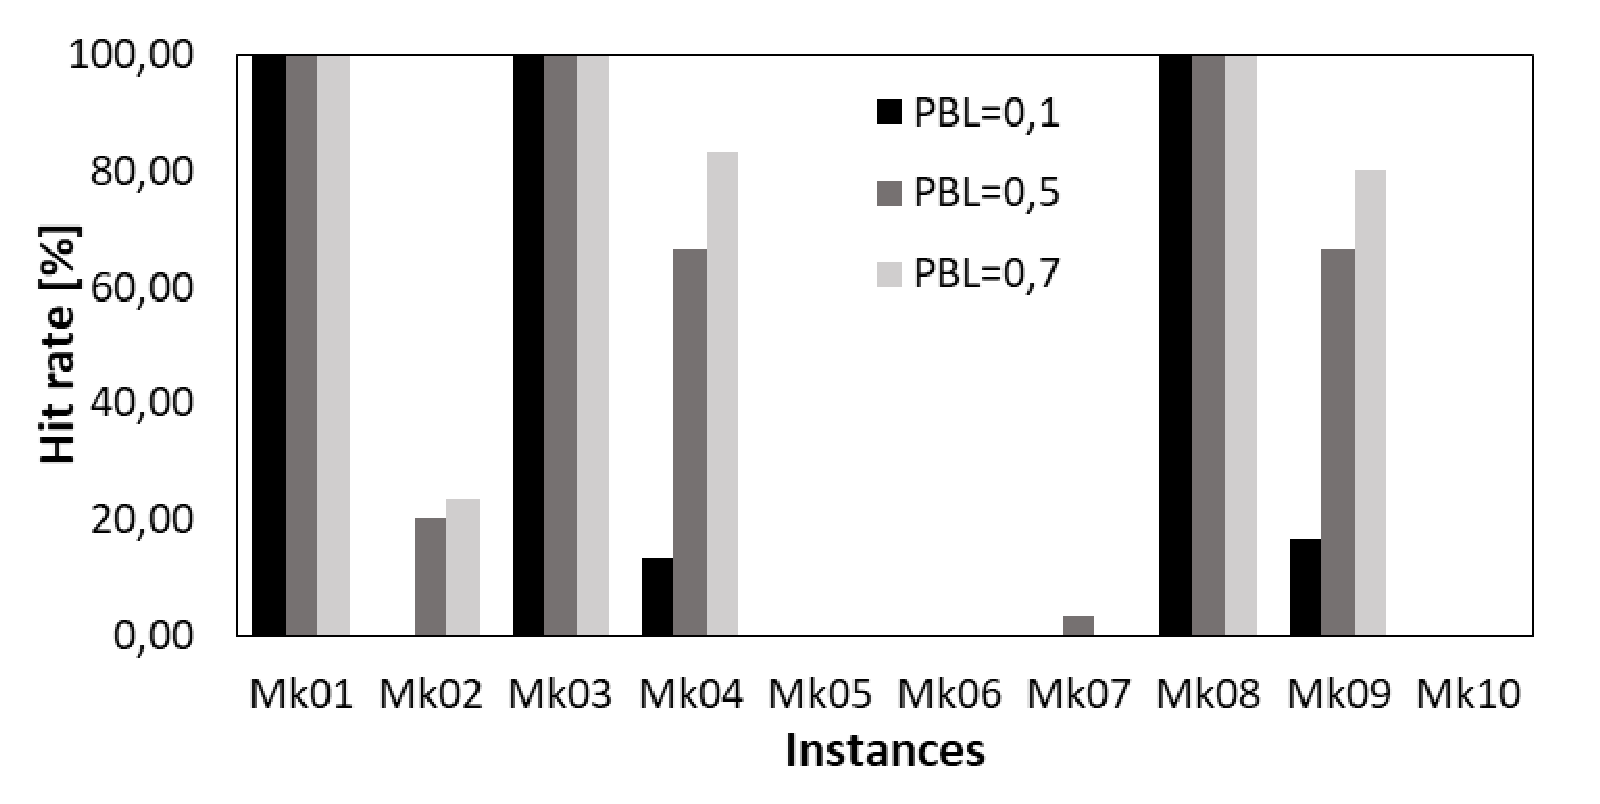
\includegraphics[width=\linewidth]{figures/DELS-hitRate.eps}
%    \caption{Hit Rate of the HDE with Different Cr values considering all FJSSP instances.}
%    \label{fig:DEhitRate}
%\end{minipage}
%\hspace{0.2cm}
\begin{minipage}[b]{0.4\linewidth}
    \centering
    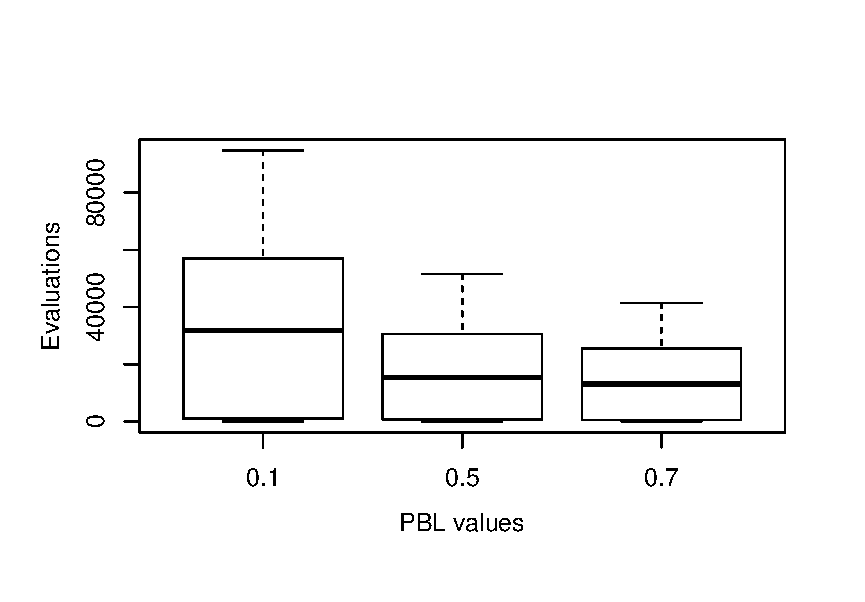
\includegraphics[width=\linewidth]{figures/DELS-Evaluations.eps}
    \vspace{-0.9cm}
    \caption{Total number of evaluations for the HDE %with different $P_{BL}$ values considering all FJSSP instances
    .}
    \label{fig:HDEevaluations}
\end{minipage}  
\hspace{0.5cm}
\begin{minipage}[b]{0.4\linewidth}
%\begin{figure}[!htb]
\scriptsize
\centering
   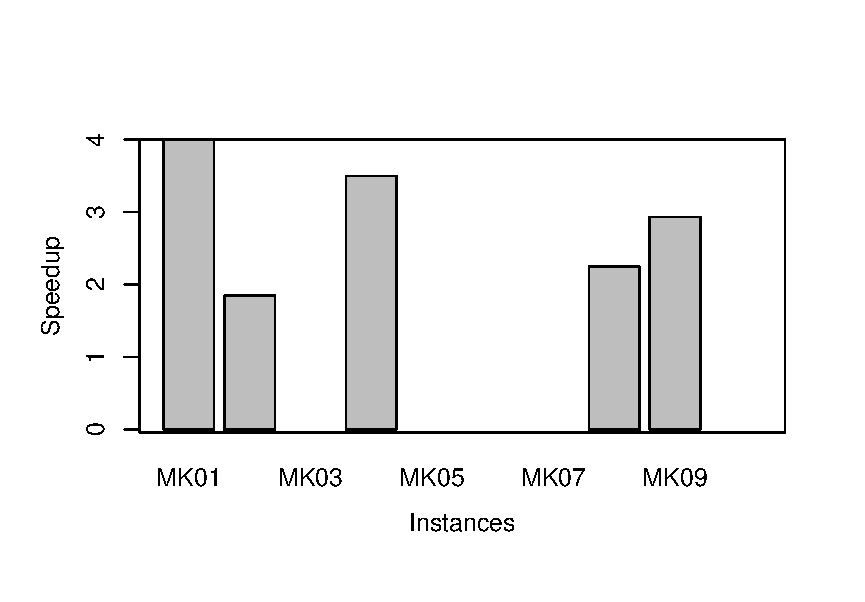
\includegraphics[width=\linewidth]{figures/speedup.eps}
   \vspace{-0.9cm}
    \caption{Speedup per FJSSP instances.}
    \label{fig:speedup}
%\end{figure}
\end{minipage}
\end{figure}


%\subsection{Results of the DE and parallelism}

%Finally, %in this section 
Following analysis is devoted to compare the HDE and its parallel version as described in Section~\ref{subsec:parallelHDE}. The most important measure of a parallel algorithm is the speedup. The speedup is defined as the ratio of the sequential execution time (HDE execution time, in this case) to the parallel execution time. For this analysis, we consider the weak speedup~\cite{albaMeta2005}. For that reason and following the best practice by Luque and Alba~\cite{Luque:2013:PGA:2564896}, the stopping criterion is based on the quality of the final solution achieved by the algorithms, which is set to the best known $C_{max}$ for each FJSSP instance (see column Opt of Table~\ref{tab:resultsDE}). Consequently, the speedup values is only reported  for the instances for which the HDE algorithm obtains the optimum value.%,as previously mentioned in previous sections.

%Once we established execution times of the HDE and the parallel HDE, we calculated the speedup values. 
Figure~\ref{fig:speedup} shows that the use of parallelization is worth while, which allow us to speed up the execution time with respect to the sequential HDE  near 3 times in average (the ideal speedup value is 4, the number of available cores per machine). 

Finally, to determine the goodness of the metaheuristics considered in this work, we present a comparison of the results from the HDE with several competitive algorithms present in the literature. This allows a comparative assessment of the algorithms for the FJSSP. In this comparison different population-based metaheuristics to solve the FJSSP are considered: i) a hybrid algorithm combining chaos particle swarm optimization with genetic algorithm (hGA)~\cite{tang2011}, ii) a bi-population based estimation of distribution algorithm (BEDA)~\cite{Wang2012917},  iii) an ant colony optimization (IACO)~\cite{WANG2017}, and finally, iv) a hybrid differential evolutionary algorithm~\cite{YUAN2013246}. From the comparison, the $C_{max}$ values of HDE are similar with the values of remaining algorithms, for the majority of the ten instances (a comparative table is no included due to lack of space). This observation suggests that the HDE developed in this work is a competitive algorithm to solve the FJSSP. Comparisons regarding computational effort are hard to be carried out because the majority of the works do not report number of evaluations. Consequently, the relative efficiency of referred algorithms are difficult to contrast in order to obtain meaningful comparisons.

\begin{table}[!tb]
\scriptsize
  \centering
  \caption{Comparison between HDE and population-based Metaheuristics from the literature}
    \begin{tabular}{l|rrrrrrrrrr|}
    \hline
    \multicolumn{1}{r}{} & \multicolumn{1}{l}{MK01} & \multicolumn{1}{l}{MK02} & \multicolumn{1}{l}{MK03} & \multicolumn{1}{l}{MK04} & \multicolumn{1}{l}{MK05} & \multicolumn{1}{l}{MK06} & \multicolumn{1}{l}{MK07} & \multicolumn{1}{l}{MK08} & \multicolumn{1}{l}{MK09} & \multicolumn{1}{l}{MK10} \\
    \hline
    HDE   & \textbf{40} & \textbf{26} & \textbf{204} & \textbf{60} & 173   & 60    & 140   & \textbf{523} & \textbf{307} & 219 \\
    hGA   & \textbf{40} & \textbf{26} & \textbf{204} & 62    & \textbf{172} & 65    & 140   & \textbf{523} & 310   & 214 \\
    BEDA  & \textbf{40} & \textbf{26} & \textbf{204} & \textbf{60} & \textbf{172} & 60    & \textbf{139} & \textbf{523} & \textbf{307} & 206 \\
    IACO  & \textbf{40} & \textbf{26} & \textbf{204} & \textbf{60} & 173   & 60    & 140   & \textbf{523} & \textbf{307} & 208 \\
    HDE   & \textbf{40} & \textbf{26} & \textbf{204} & \textbf{60} & \textbf{172} & \textbf{57} & \textbf{139} & \textbf{523} & \textbf{307} & \textbf{198} \\
\hline
    \end{tabular}%
  \label{tab:addlabel}%
\end{table}%
